%\documentclass[10pt,notes]{beamer}       % print frame + notes
%\documentclass[10pt, notes=only]{beamer}   % only notes
\documentclass[11pt]{beamer}              % only frames

%%%%%% IF YOU WOULD LIKE TO CREATE LECTURE NOTES COMMENT OUT THE FOlLOWING TWO LINES
%\usepackage{pgfpages}
%\setbeameroption{show notes on second screen=bottom} % Both

\usepackage{graphicx}
\DeclareGraphicsExtensions{.pdf,.png,.jpg}
\usepackage{color}
\usetheme{winslab}
\usepackage[utf8]{inputenc}
\usepackage[english]{babel}
\usepackage{amsmath}
\usepackage{amsfonts}
\usepackage{amssymb}




\usepackage{algorithm2e,algorithmicx,algpseudocode}
\algnewcommand\Input{\item[\textbf{Input:}]}%
\algnewcommand\Output{\item[\textbf{Output:}]}%
\newcommand\tab[1][1cm]{\hspace*{#1}}

\algnewcommand{\Implement}[2]{\item[\textbf{Implements:}] #1 \textbf{Instance}: #2}%
\algnewcommand{\Use}[2]{\item[\textbf{Uses:}] #1 \textbf{Instance}: #2}%
\algnewcommand{\Trigger}[1]{\Statex{\textbf{Trigger:} (#1)}}%
\algnewcommand{\Events}[1]{\item[\textbf{Events:}] #1}%
\algnewcommand{\Need}[1]{\item[\textbf{Needs:}] #1}%
\algnewcommand{\Event}[2]{\Statex \item[\textbf{On#1:}](#2) \textbf{do}}%
\algnewcommand{\Trig}[3]{\State \textbf{Trigger}  #1.#2 (#3) }%
\def\true{\textbf{T}}
\def\false{\textbf{F}}


\author[İmre KOSDİK]{İmre KOSDİK\\\href{mailto:imre.kosdik@metu.edu.tr}{imre.kosdik@metu.edu.tr}}
%\author[J.\,Doe \& J.\,Doe]
%{%
%  \texorpdfstring{
%    \begin{columns}%[onlytextwidth]
%      \column{.45\linewidth}
%      \centering
%      John Doe\\
%      \href{mailto:john@example.com}{john@example.com}
%      \column{.45\linewidth}
%      \centering
%      Jane Doe\\
%      \href{mailto:jane.doe@example.com}{jane.doe@example.com}
%    \end{columns}
%  }
%  {John Doe \& Jane Doe}
%}

\title[Termination and Deadlock Detection]{Termination  and Deadlock Detection in Distributed Systems}
\subtitle[Short SubTitle]{Shavit-Francez Termination Detection Algorithm & Bracha-Toueg Deadlock Detection Algorithm}
\date{} 

\begin{document}

\begin{frame}[plain]
\titlepage
\note{In this talk, I will present the two algorithms utilized for termination and deadlock detection in distributed systems. After the talk, I hope you will gain insight into the implementation details of these algorithms and analyze their performance from the message and time complexity perspective from the experimentation results. Both the termination and deadlock issues are widespread not only in distributed systems but also in the operating systems of our computers. From the operating system perspective, a deadlock is a condition where processes wait for each other indefinitely in a cyclic manner. Handling deadlocks is an intriguing and substantial issue in utilizing the system resources efficiently and preventing performance degradation. We say that a process terminates when it finishes its computation and is ready to perform its remaining tasks. Detecting the process termination is critical in the same sense as deadlock detection because processes may depend on others to finish their execution to use their outputs or the resources they used. These concepts we are familiar with in the operating systems area apply to distributed systems. Therefore, understanding and employing these algorithms in distributed systems is prominent. 
\begin{enumerate}
\item Why are you giving presentation?
\item What is your desired outcome?
\item What does the audience already know  about your topic?
\item What are their interests?
\item What are key points?
\end{enumerate}
}
\end{frame}

\begin{frame}[label=toc]
    \frametitle{Outline of the Presentation}
    \tableofcontents[subsubsectionstyle=hide]
\note{ Here is my outline for the presentation. Since I have two distinct algorithms, I plan to explain the details of both the algorithms on each section. 
\begin{enumerate}
\item Outline 
\item The Deadlock and Termination Detection Problems
\item The Related Works and Background Research on Deadlock and Termination Detection
\item My Contribution on Deadlock Detection and Termination Detection Algorithms
\item The Results of Experiments on Deadlock Detection and Termination Detection
\item Conclusion and Recommendations 
\end{enumerate}
}
\end{frame}
%
%\part{This the First Part of the Presentation}
%\begin{frame}
%        \partpage
%\end{frame}
%
\section{The Problem of Deadlock Detection And Termination Detection}
%\begin{frame}
%        \sectionpage
%\end{frame}

\begin{frame}{The Problem of Deadlock Detection}
%\framesubtitle{Tell a \alert{STORY} from the background to the conclusion}

\begin{figure}
    \centering
    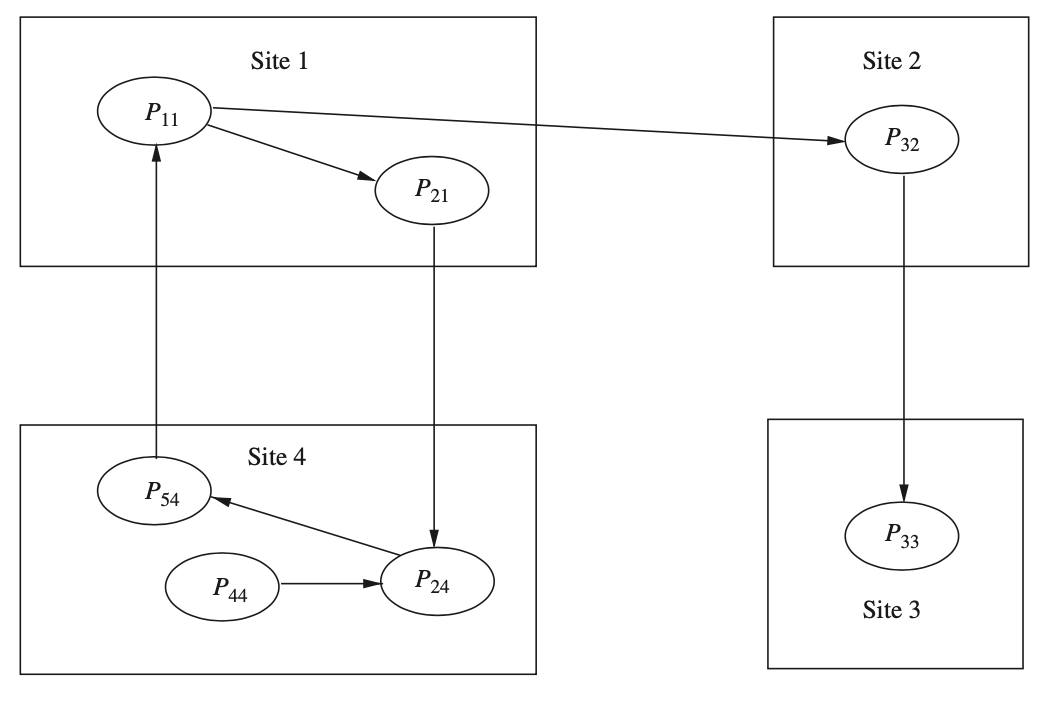
\includegraphics[scale=0.25]{figures/deadlock.png}
    \caption{Distributed System with Deadlocks}
    \label{fig:distributed_system_with_deadlocks}
\end{figure}

\begin{block}{Deadlock Detection} 
Deadlock is a state where processes in a distributed system wait indefinitely for each other to allocate resources to perform their computations. Deadlock detection requires analyzing the running system for cyclic dependencies.
\end{block}

\note{Deadlock Detection: Processes need resources to perform their computations. However, the resources may not always be available because another process may be using them at that time. In such a case, the process needs to wait for another process to release its resources. Sometimes, this wait becomes cyclic, and none of the processes can continue execution because they cannot allocate resources. This system state is the deadlock state in a distributed system. Therefore, to detect the deadlocks, we need to look for cyclic dependencies in the system. For example, in the figure, there is a cyclic dependency in P11, P21, P34 and P54. Deadlock detection is a fundamental problem because none of the processes are aware of the global system state, and processes do not share any global clock.}
\end{frame}

\begin{frame}{The Problem of Termination Detection}

\begin{block}{Termination Detection} 
Termination detection is the problem of determining if a distributed computation has terminated. A distributed system terminates when all its processes become passive with no messages in transit. Termination detection requires a particular process (or all of the processes) to infer when the underlying computation has terminated.
\end{block}
%Spend at least \textbf{1.5-2 minutes per slide} on average.

%The introduction should be something like ``I will be presenting title of talk. This is joint work with your colleagues or advisor at institution.'' 

\note{Termination Detection: Termination detection is the problem of determining whether a distributed computation has terminated. Processes can be either in an active state or in a passive state. We say that a distributed computation terminates when all the processes transition to a passive state and no messages are in transit. Determining the termination requires one or more processes to infer when the computation has terminated. Termination detection is a fundamental problem in the same sense as the deadlock detection problem. Additionally, processes may reactivate each other by sending messages. This issue increases the challenge.}

\end{frame}

\section{The Contributions}
\begin{frame}
\frametitle{Contributions To The Deadlock Detection and Termination Detection Algorithms}
\framesubtitle{}
\begin{itemize}
\item Implementation of Shavit-Francez termination detection algorithm on AHCv2 platform
\item Performance analysis of Shavit-Francez algorithm
\item Implementation of Bracha-Toueg deadlock detection algorithm on AHCv2 platform
\item Performance analysis of Bracha-Toueg algorithm
\end{itemize}

\note{As a contribution, I implemented both of the algorithms using the AHC library and conducted different experiments on my implementations to analyze the performance of both algorithms in terms of message and time complexity.}
\end{frame}


\section{Motivation/Importance}
\begin{frame}
\frametitle{Motivation/Importance of Detecting Termination}
\framesubtitle{Shavit-Francez Termination Detection Algorithm}
\begin{itemize}
\item Crucial to determine which processes terminated execution since other processes depend on their outputs.
\item Achieving a \textbf{consistent} system state which results in preserving the \textbf{correctness} of the system.
\item Efficient resource utilization with the possibility of preventing \textbf{deadlocks}.
\item A significant challenge because processes do not share a \textbf{global clock} and do not have the knowledge of the \textbf{global state} of the system.
\end{itemize}

\end{frame}

\begin{frame}
\frametitle{Motivation/Importance of Detecting Deadlocks}
\framesubtitle{Brahca-Toueg Deadlock Detection Algorithm}
\begin{itemize}
\item Prevent system failures resulting in increased \textbf{reliability}.
\item Prevent waste of resources to positively affect system's \textbf{response} time and \textbf{throughput}.
\item A significant challenge because processes do not share a \textbf{global clock} and do not have the knowledge of the \textbf{global state} of the system.
\item \textbf{Lack of shared memory} causes issues related to constructing and maintaining the system state graph which the algorithm runs on.
\end{itemize}
\end{frame}

\section{Background/Model/Definitions/Previous Works}


\subsection{Model, Definitions}

\frame{
\frametitle{Model and Definitions for Deadlock Detection}

\begin{block}{Definitions} 
\begin{itemize}
\item \textbf{N-out-of-M Requests Deadlock Model}: A process makes M requests and can continue execution only if it obtains at least N resources.
\item \textbf{Wait-For-Graph (WFG):} A graph modeling the resource or communication dependencies. Nodes are processes, and there is a directed edge from one node to another if the first node waiting to acquire a resource that the second one is currently holding. 
\end{itemize}
\end{block}
}

\frame{
\frametitle{Model and Definitions for Deadlock Detection}
\begin{figure}
    \centering
    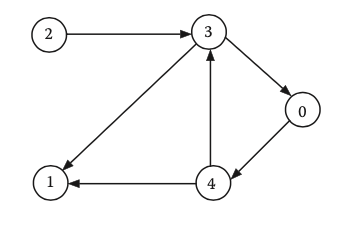
\includegraphics[scale=0.3]{figures/deadlock2.png}
    \caption{Distributed System with Deadlocks}
    \label{fig:distributed_system_with_deadlocks2}
\end{figure}
\begin{block}{Definitions} 
\begin{itemize}
\item \textbf{Active Process:} Process that holds all the resources it needs and is either executing or ready to execute.
\item \textbf{Blocked Process:} Process waiting to acquire the resources it needs. An active process becomes blocked once it sends an N-out-of-M request and remains blocked until at least N of the resources are granted to it.
\end{itemize}
\end{block}
}

\frame{
\frametitle{Model and Definitions for Termination Detection}

\begin{block}{Definitions} 
\begin{itemize}

\end{itemize}
\end{block}
}


\subsection{Background, Previous Works}
\begin{frame}{Background}

\end{frame}




\section{Contribution}
\subsection{Main Point 1}
\begin{frame}{Main Point 1: A Figure}
\framesubtitle{Abstract the Major Results}
Describe the key results of the paper. You may present the statements of the major theorems, but not their proofs. You will probably have to get a little technical here, but do so gradually and carefully.

\begin{figure}
    \centering
    
\includegraphics[scale=0.5]{figures/Chick1.png}
    \caption{Awesome Image}
    \label{fig:awesome_image}
\end{figure}
\note{
}
\end{frame}


\subsection{Main Point 2}

\begin{frame}
\frametitle{An Example Distributed Algorithm}
\framesubtitle{Blind Flooding}


Blind flooding on an undirected graph is presented in Algorithm~\ref{alg:blindflooding}.

\begin{center}
\begin{algorithm}[H]
	\scriptsize
	\def\algorithmlabel{BlindFlooding}
    \caption{\algorithmlabel\ algorithm}
    \label{alg:blindflooding}
    \begin{algorithmic}[1]
    	\Implement {\algorithmlabel}{cf} 
    	\Use {LinkLayerBroadcast} {lbc} 
    	\Events{Init, MessageFromTop, MessageFromBottom}
	\Need {}

        \Event {Init}{}
        		
        \Event{MessageFromBottom} { $m$ }
        		\Trig{lbc}{Broadcast} { $m$  }
        		
        \Event{MessageFromTop} { $m$ }	
        		\Trig{lbc}{Broadcast} { $m$  }
    \end{algorithmic}
\end{algorithm}
\end{center}


\end{frame}

\begin{frame}
\frametitle{Main Point 2}
\framesubtitle{Explain the Significance of the Results}
Pause, and explain the relationships between the formal theorems that you have just presented and the informal description that you gave in the Introduction. Make it clear to the audience that the results do live up to the advance publicity. If the statements of the theorems are very technical then this may take some time. It is time well-spent.

\end{frame}

\subsection{Main Point 3}
\begin{frame}
\frametitle{Main Point 3}
\framesubtitle{Sketch a Proof of the Crucial Results}
The emphasis is on the word ``sketch''. Give a very high-level description of the proofs, emphasizing the proof structure and the proof techniques used. If the proofs have no structure (in which case it may be assumed that you are not the author of the paper), then you must impose one on them. Gloss over the technical details. It is a good idea to point them out but not to explore them.
\end{frame}


\section{Experimental results/Proofs}

\subsection{Main Result 1}
\begin{frame}
\frametitle{Main Result 1}
\framesubtitle{}
Choose \textbf{just the key results}. They should be important, non-trivial, should give the flavour of the rest of the technical details and should be presentable in a relatively short period of time. Use figures instead of tables instead of text.

Better to present 10\% the entire audience gets than 90\% nobody gets
\end{frame}


\subsection{Main Result 2}
\begin{frame}
\frametitle{Main Result 2}
\framesubtitle{Try a subtitle}
\begin{itemize}
\item Make sure your notation is clear and consistent throughout the talk. Prepare a slide that explains the notation in detail, in case that is needed or if somebody asks.
\item Always label all of your axes on graphs; use short but helpful captions on figures and tables. It is also very useful to have an arrow on the side which clearly shows which direction is considered better (e.g., "up is better").
\item If you have experimental results, make sure you clearly present the experimental paradigm you used, and the details of your methods, including the number of trials, the specific analysis tools you applied, significance testing, etc.
\item The talk should contain at least a brief discussion of the limitations and weaknesses of the presented approach or results, in addition to their strengths. This, however, should be done in an objective manner -- don't enthusiastically put down your own work.
\end{itemize}
\end{frame}


\subsection{Main Result 3}
\begin{frame}
\frametitle{Main Result 3}
\framesubtitle{}
\begin{itemize}
\item If time allows, the results should be compared to the most related work in the field. You should at least prepare one slide with a summary of the related work, even if you do not get a chance to discuss it. This will be helpful if someone asks about it, and will demonstrate your mastery of the material.
\item Spell check again.
\item Give for each of the x-axis, y-axis, and z-axis
\item Label, unit, scale (if log scale)
\item Give the legend
\item Explain all symbols
\item Take an example to illustrate a specific point in the figure
\end{itemize}
\end{frame}



\section{Conclusions}
\begin{frame}
\frametitle{Conclusions}
\framesubtitle{Hindsight is Clearer than Foresight}
Advices come from \cite{spillman2000present}.
\begin{itemize}
\item You can now make observations that would have been confusing if they were introduced earlier. Use this opportunity to refer to statements that you have made in the previous three sections and weave them into a coherent synopsis. You will regain the attention of the non- experts, who probably didn’t follow all of the Technicalities section. Leave them feeling that they have learned something nonetheless.
\item Give Open Problems It is traditional to end with a list of open problems that arise from your paper. Mention weaknesses of your paper, possible generalizations, and indications of whether they will be fruitful or not. This way you may defuse antagonistic questions during question time.
\item Indicate that your Talk is Over
An acceptable way to do this is to say “Thank-you. Are there any questions?”\cite{einstein}
\end{itemize}

\end{frame}

\section*{References}
\begin{frame}{References}
\tiny
\bibliographystyle{IEEEtran}
\bibliography{refs}
\end{frame}

\begin{frame}{How to prepare the talk?}
Please read \url{http://larc.unt.edu/ian/pubs/speaker.pdf}
\begin{itemize}
\item The Introduction:  Define the Problem,    Motivate the Audience,    Introduce Terminology,    Discuss Earlier Work,    Emphasize the Contributions of your Paper,    Provide a Road-map.
\item The Body:    Abstract the Major Results, Explain the Significance of the Results, Sketch a Proof of the Crucial Results
\item Technicalities: Present a Key Lemma, Present it Carefully
\item The Conclusion: Hindsight is Clearer than Foresight, Give Open Problems, Indicate that your Talk is Over
\end{itemize}

\note{
\begin{itemize}
\item The Introduction:  Define the Problem,    Motivate the Audience,    Introduce Terminology,    Discuss Earlier Work,    Emphasize the Contributions of your Paper,    Provide a Road-map.
\item The Body:    Abstract the Major Results, Explain the Significance of the Results, Sketch a Proof of the Crucial Results
\item Technicalities: Present a Key Lemma, Present it Carefully
\item The Conclusion: Hindsight is Clearer than Foresight, Give Open Problems, Indicate that your Talk is Over 
\end{itemize}
}
\end{frame}



\thankslide




\end{document}